\documentclass[a4paper, 11pt]{article}
\usepackage{geometry}
\usepackage{graphicx}
\usepackage{a4wide}
\usepackage{ulem}
\usepackage{amsthm}
\usepackage{amsmath}
\usepackage{amsfonts}
\usepackage{amssymb}
\usepackage[T1]{fontenc}
\usepackage{ngerman}
\usepackage{graphicx}
\usepackage{epic}
\usepackage{enumerate}
\usepackage{tabu}
\usepackage [latin1]{inputenc}
\geometry{a4paper,left=15mm,right=25mm,top=20mm,bottom=25mm}
%\renewcommand{\baselinestretch}{1.5}
\newcommand{\ol}{\overline}
\newcommand{\makeline}{\hrule\vspace{5pt}}
\newcommand{\ip}[2]{\left< #1, #2 \right>}

\title{6. �bungsblatt zu Software Qualit�t}
\author{Michel Meyer, Manuel Schwarz}

\begin{document}
  \maketitle

  \section*{Aufgabe 7.1}
  \subsection*{(a)}
  %\begin{figure}
		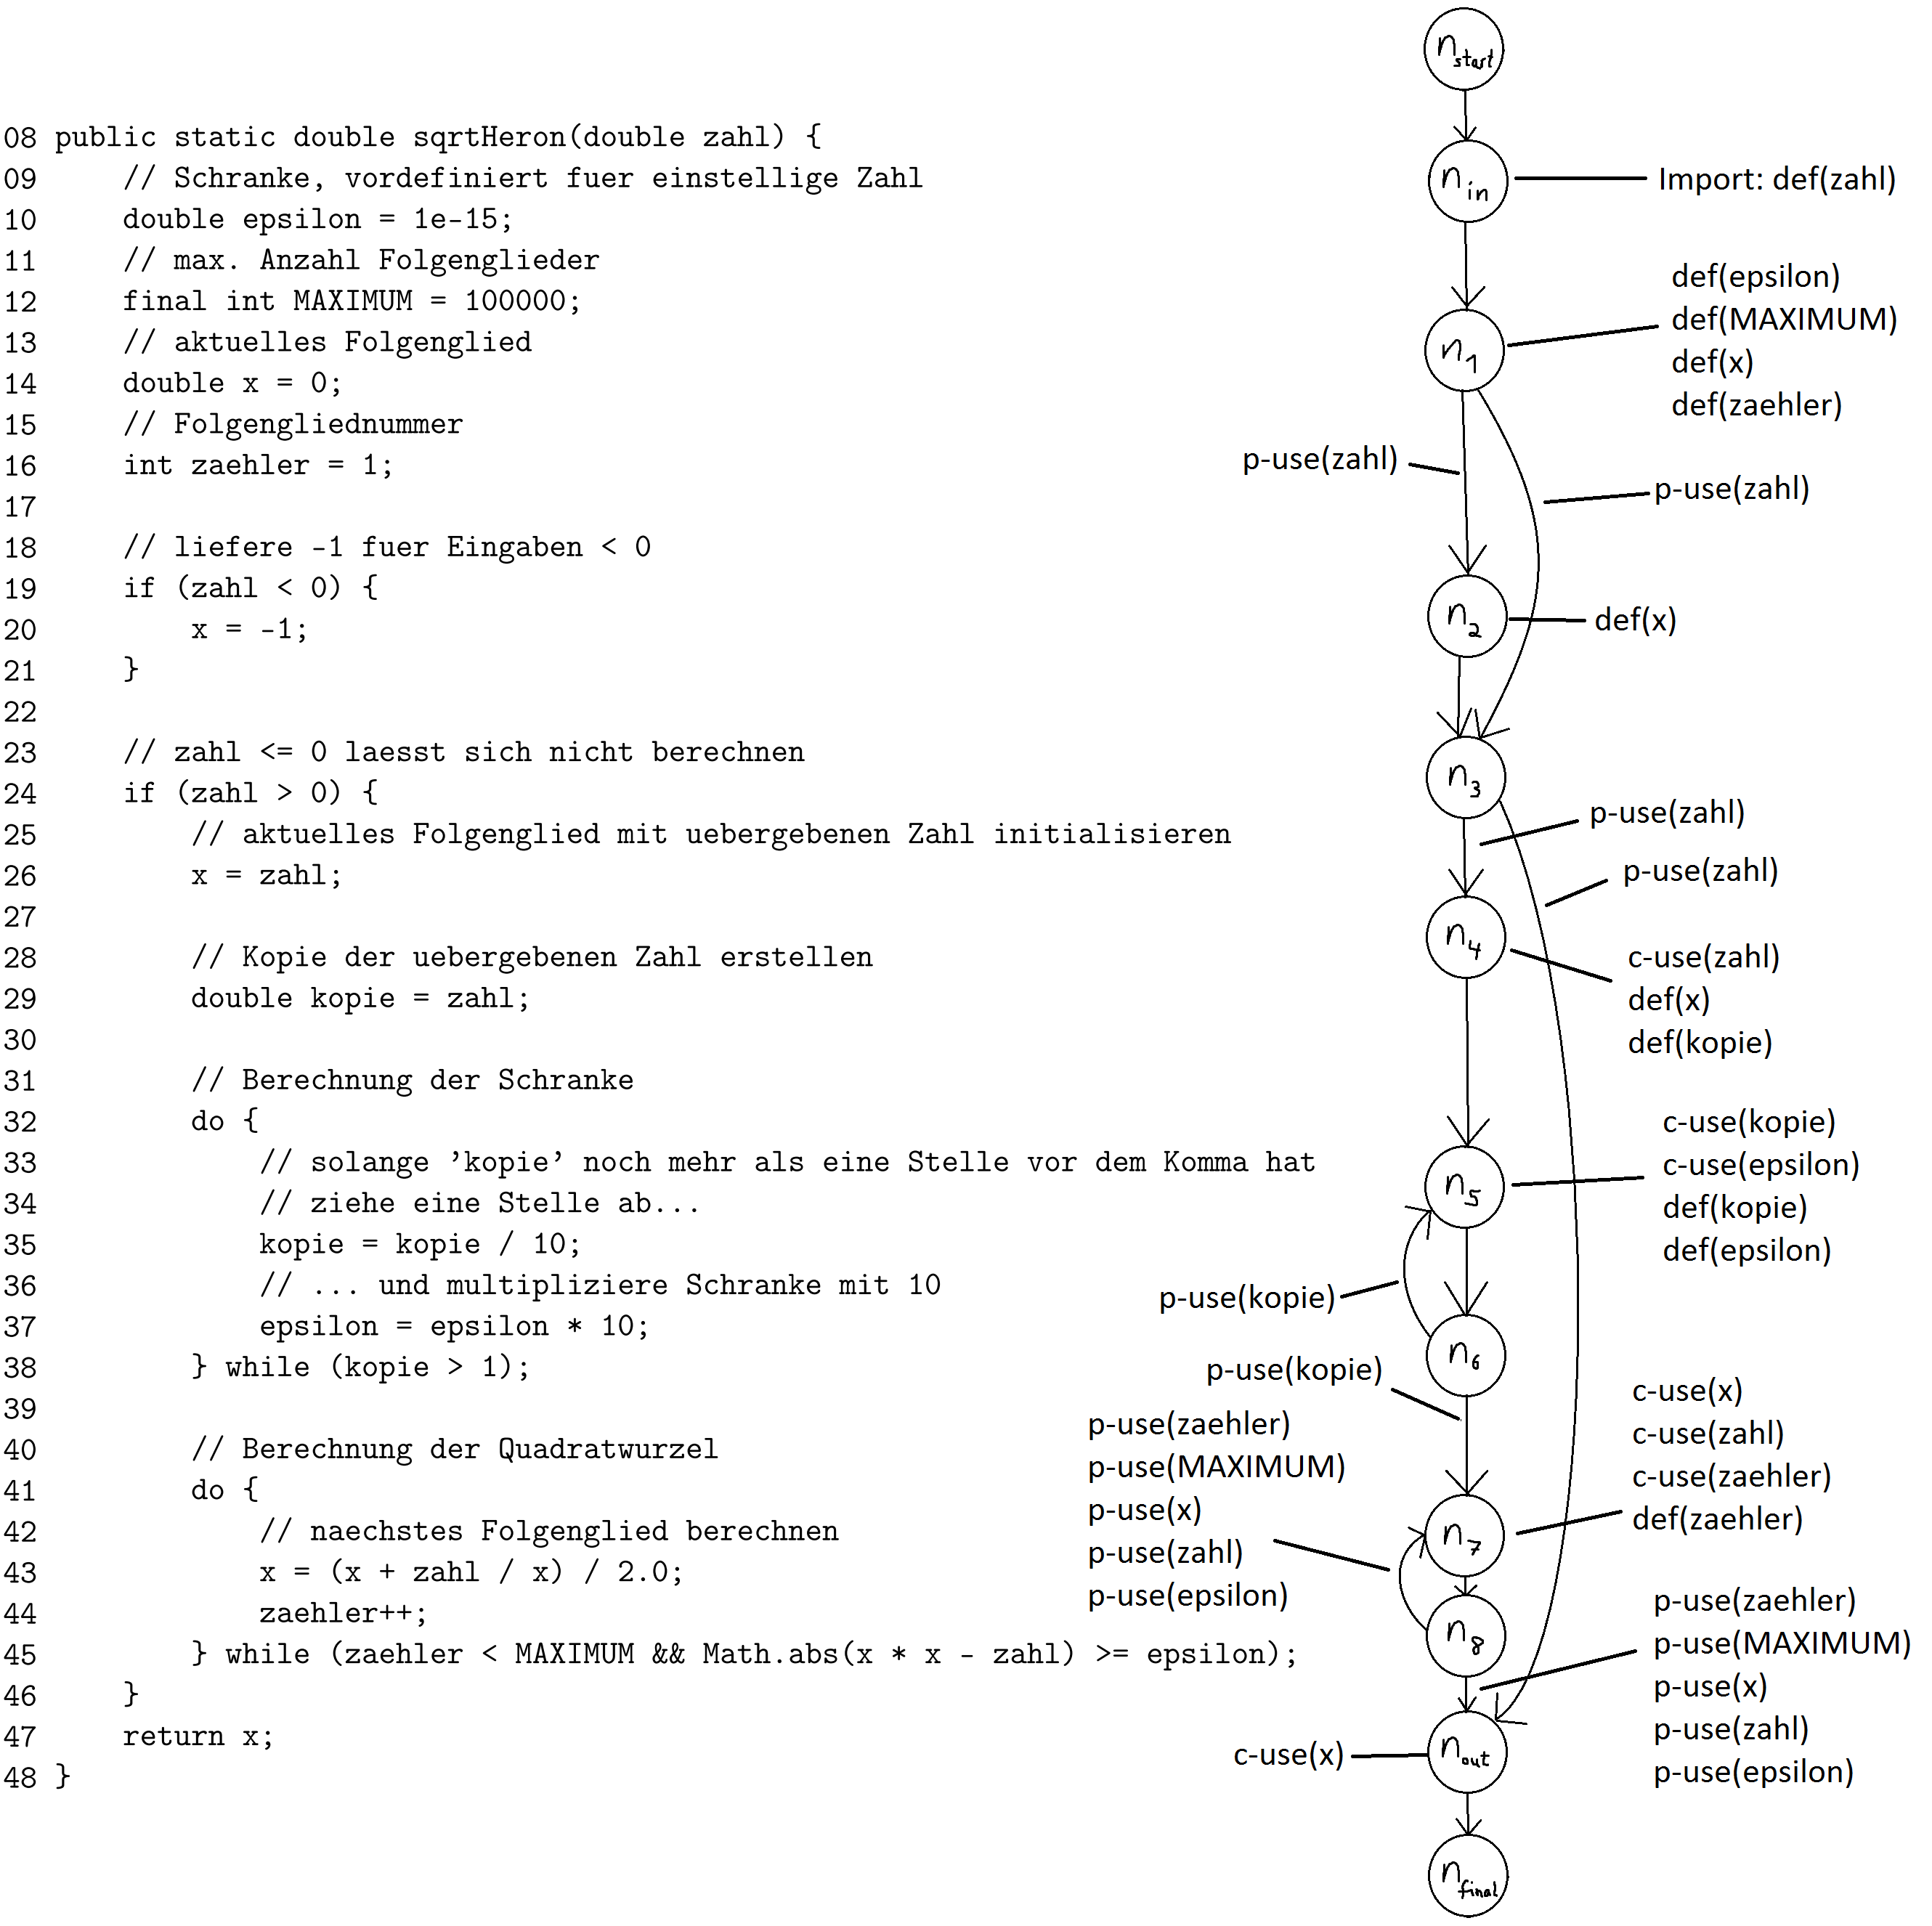
\includegraphics[width=\columnwidth]{Aufg1a.png}
	%\end{figure}
	\newpage
	\subsection*{\textit{dcu} und \textit{dpu}}
	\begin{tabular}{|l|l|l|l|}\hline
		\textbf{Variable} & \textbf{Knoten $n_i$} & \textbf{\textit{dcu($x, n_i$)}} & \textbf{\textit{dpu($x, n_i$)}} \\\hline\hline
		\texttt{zahl}    & $n_{in}$ & \{$n_4, n_7$\}& \{$(n_1, n_2), (n_1, n_3), (n_3, n_4), (n_3, n_{out}), (n_8, n_7), (n_8, n_{out})$\} \\\hline
		\texttt{epsilon} & $n_1$    & \{$n_5$\}     & \{$$\} \\\hline
		\texttt{epsilon} & $n_5$    & \{$n_5$\}     & \{$$\} \\\hline
		\texttt{MAXIMUM} & $n_1$    & \{$$\}        & \{$$\} \\\hline
		\texttt{x}       & $n_1$    & \{$n_{out}$\} & \{$$\} \\\hline
		\texttt{x}       & $n_2$    & \{$n_{out}$\} & \{$$\} \\\hline
		\texttt{x}       & $n_4$    & \{$n_7$\}     & \{$$\} \\\hline
		\texttt{zaehler} & $n_1$    & \{$n_7$\}     & \{$$\} \\\hline
		\texttt{zaehler} & $n_7$    & \{$n_7$\}     & \{$$\} \\\hline
		\texttt{kopie}   & $n_4$    & \{$n_5$\}     & \{$$\} \\\hline
		\texttt{kopie}   & $n_5$    & \{$n_5$\}     & \{$$\} \\\hline
	\end{tabular}
	
  \subsection*{(b) \textit{All-defs}}
		Die Menge
		\begin{align*}
			\{(n_{start}, n_{in}, n_1, n_2, n_3, n_4, n_5, n_6, n_7, n_8, n_{out}, n_{final})\}
		\end{align*}
		testet alle definierten Variablen mindestens einmal mit \textit{c-use} oder \textit{p-use}.
	\subsection*{(c) \textit{All-p-uses}}
		Die Menge
		\begin{align*}
			\{ & (n_{start}, n_{in}, n_1, n_2, n_3, n_4, n_5, n_6, n_7, n_8, n_{out}, n_{final}), \\
			   & (n_{start}, n_{in}, n_1, n_3, n_{out}, n_{final}), \\
			   & (n_{start}, n_{in}, n_1, n_3, n_4, n_5, n_6, n_5, n_6, n_7, n_8, n_7, n_8, n_{out}, n_{final})\}
		\end{align*}
		testet zu allen definierten Variablen alle \textit{p-use}s.
\end{document}
